\begin{lrbox}{\lstlistingIn}
   \begin{lstlisting}[style=c++,backgroundcolor={}]
`\clingPrompt` puts("Hello, world!");
   \end{lstlisting}
\end{lrbox}
\begin{lrbox}{\lstlistingWrap}
   \begin{lstlisting}[style=c++,backgroundcolor={}]
void __cling_Un1Qu30(void *) {
    puts("Hello, world!");
}
   \end{lstlisting}
\end{lrbox}
\begin{lrbox}{\lstlistingCodeGen}
  \begin{lstlisting}[language=llvm]
@.str = private unnamed_addr constant [14 x i8] c"Hello, world!\00", align 1

; Function Attrs: nofree nounwind sspstrong uwtable
define dso_local void @__cling_Un1Qu30(ptr nocapture noundef readnone %0) local_unnamed_addr {
  %2 = tail call i32 @puts(ptr noundef nonnull dereferenceable(1) @.str)
  ret void
}
  \end{lstlisting}
\end{lrbox}

\tikz[start chain=c going below,node distance=15pt,
  every node/.style={font=\scriptsize},
  every on chain/.style={join=by ->},
  rect/.style={top color=white,bottom color=teal!50!black!20,draw=teal!50!black!50,text width=1.75in,align=center,minimum height=20pt,inner sep=1pt,rounded corners},
  expl line/.style={dotted,black!25,->},
  expl/.style={draw,black,densely dotted,fill=white,font={\ttfamily\scriptsize},text width=2.5in}]{

  \def\ASTpre{\tikz\graph[tree layout,level distance=4pt,sibling distance=4pt,nodes={circle,inner sep=1.5pt,as=,fill=black}]{ a -- { b, c }};}
  \def\ASTpost{\tikz\graph[tree layout,level distance=4pt,sibling distance=4pt,nodes={circle,inner sep=1.5pt,as=,fill=black}]{ a -- { b -- { c, d }, e -- f }};}
  \def\sepRule{\rule{27pt}{0pt}}

  \begin{scope}[every node/.append style=on chain]
    \path node(in) {User input}
    node(wrap)[rect] {Wrap top-level statements}
    node(parse)[rect] {Parse (clang)}
    node(transform)[rect] {AST transformers}
    node(codegen)[rect] {Code generation}
    node(callwrapper)[rect] {Call wrapper function\\(if any)};
  \end{scope}

  % Step-by-step explanation
  \draw<1->[expl line] (in) -- ++(right:2in) node(in_expl)[at end,anchor=west,expl]{%
    \usebox{\lstlistingIn}
  };
  \draw<2->[expl line] (wrap) -- ++(right:2in) node(wrap_expl)[at end,anchor=west,expl]{%
    \usebox{\lstlistingWrap}
  };
  \draw<3->[expl line] (parse) -- ++(right:2in) node(parse_expl)[at end,anchor=west,expl]{%
    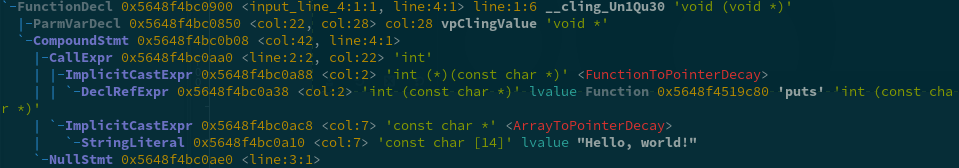
\includegraphics[width=\textwidth]{img/clang-ast-expl.png}
  };
  \draw<4->[expl line] (transform) -- ++(right:2in) node(transform_expl)[at end,anchor=west,black,solid]{%
    \ASTpre \sepRule $\rightarrow$ \sepRule \ASTpost
  };
  \draw<5->[expl line] (codegen) -- ++(right:2in) node(codegen_expl)[at end,anchor=west,expl]{%
    \resizebox{\textwidth}{!}{\usebox{\lstlistingCodeGen}}
  };
  \draw<6->[expl line] (callwrapper) -- ++(right:2in) node(callwrapper_expl)[at end,anchor=west,expl]{%
    [If $\exists$ top-level statement, get a pointer to the wrapper function and do indirect call]
  };

}
